\documentclass[11pt]{article}
\usepackage[utf8]{inputenc}     % for éô
\usepackage{charter}
\usepackage[english]{babel}     % for proper word breaking at line ends
% \usepackage[a4paper, left=1.5in, right=1.5in, top=1.5in, bottom=1.5in]{geometry}
                                % for page size and margin settings
\usepackage{graphicx}           % for ?
\usepackage{amsmath,amssymb}    % for better equations
\usepackage{amsthm}             % for better theorem styles
\usepackage{mathtools}          % for greek math symbol formatting
\usepackage{enumitem}           % for control of 'enumerate' numbering
\usepackage{listings}           % for control of 'itemize' spacing
\usepackage{todonotes}          % for clear TODO notes
\usepackage[colorlinks=true, allcolors=black]{hyperref}  % page numbers and '\ref's become clickable
\usepackage{svg}
\usepackage[font=small, labelfont=bf]{caption}
\usepackage{subfig}
\usepackage{tikz}
\usepackage{bm}
\usepackage{algorithm}
\usepackage{algpseudocode}

% Set page size and margins
% Replace `letterpaper' with`a4paper' for UK/EU standard size
\usepackage[a4paper,top=2cm,bottom=2cm,left=3cm,right=3cm,marginparwidth=1.75cm]{geometry}
\usetikzlibrary{decorations.pathreplacing,calligraphy}
% To see linewidth and/or textwidth
% \usepackage{layouts}

% TEMPORARY no figures for fast building
\makeatletter
  \AtBeginDocument{%
    \def\Ginclude@graphics#1{%
      \begingroup\fboxsep=-\fboxrule
      \fbox{\rule{\@ifundefined{Gin@@ewidth}{150pt}{\Gin@@ewidth}}{0pt}%
        \rule{0pt}{\@ifundefined{Gin@@eheight}{100pt}{\Gin@@eheight}}}\endgroup}}
\makeatother

% Graphicspath
\graphicspath{ {./images/} }

% Definitions
\def\thesistitle{Noise-induced replay in\\ shallow autoencoders}
\def\thesissubtitle{Learning by dreaming}
\def\thesisauthorfirst{Jelmar}
\def\thesisauthorsecond{Gerritsen}
\def\thesissupervisorfirst{dr. Francesco}
\def\thesissupervisorsecond{Battaglia}
\def\thesissupervisorreaderfirst{dr. Federico}
\def\thesissupervisorreadersecond{Stella}
\def\thesissecondreaderfirst{prof. dr. Bert}
\def\thesissecondreadersecond{Kappen}
\def\thesisdate{July 2021}

%% THEOREM STYLES
\newtheorem{theorem}{Theorem}[section]

% \theoremstyle{definition}
\newtheorem*{definition}{Definition}

\theoremstyle{remark}
\newtheorem*{remark}{Remark}

% Title
\title{\thesistitle}
\author{\thesisauthorfirst\space\thesisauthorsecond}
\date{\thesisdate}

% Todos
\newcommand{\towrite}[1]{\todo[inline,color=yellow!10]{TO WRITE: #1}}
% Given
\newcommand\given[1][]{\:#1\vert\:}

\begin{document}

% Title page
\begin{titlepage}
  \thispagestyle{empty}
  \newcommand{\HRule}{\rule{\linewidth}{0.5mm}}
  \center
  \textsc{\Large Radboud University Nijmegen}\\[.7cm]
  \includegraphics[width=25mm]{in_dei_nomine_feliciter.eps}\\[.5cm]
  \textsc{Faculty of Science}\\[0.5cm]

  \HRule \\[0.4cm]
  { \huge \bfseries \thesistitle}\\[0.1cm]
  \textsc{\thesissubtitle}\\
  \HRule \\[.5cm]
  \textsc{\large Thesis BSc Physics \& Astronomy}\\[.5cm]
  {\large \thesisdate}\\[.5cm]

  \begin{minipage}{0.4\textwidth}
    \begin{flushleft} \large
      \emph{Author:}\\
      \thesisauthorfirst\space \textsc{\thesisauthorsecond}
    \end{flushleft}
  \end{minipage}
  ~
  \begin{minipage}{0.4\textwidth}
    \begin{flushright} \large
      \emph{First supervisor:} \\
      \thesissupervisorfirst\space \textsc{\thesissupervisorsecond} \\[1em]
      \emph{Daily supervisor \& First reader:} \\
      \thesissupervisorreaderfirst\space \textsc{\thesissupervisorreadersecond} \\[1em]
      \emph{Second reader:} \\
      \thesissecondreaderfirst\space \textsc{\thesissecondreadersecond}
    \end{flushright}
  \end{minipage}\\[4cm]
  \vfill
  % {\large \thesisdate}\\
  \clearpage
\end{titlepage}

% Abstract
\begin{abstract}
  It is well-known that the mammalian brain is able to replay past experiences, an ability which has been linked to the hippocampus and one which appears to be important for memory consolidation. However, the reactivated neural patterns are not always exactly the same as when they originally occurred, and they can even represent novel activations that were never experienced in the first place.

  We aim to get a better understanding of replay and its potential mechanisms through the use of artificial neural networks. Specifically, a denoising autoencoder is trained in an unsupervised manner to reconstruct a hierarchical toy dataset, whose latent space is then analyzed using methods from attractor dynamics. When a trained model is initially fed random noise and its outputs are continually looped-back to serve as input for the next iteration, fixed-point attractor states can be observed. We show that the patterns produced by this iterative process can be reliably used to train a second model to reproduce the original dataset, which it is never trained on directly. We evaluate the
  behavior and feasibility of models trained in this manner, and discuss its potential implications for the nature of replay.
\end{abstract}

\vspace{.3cm}

\small{\textbf{Keywords:} machine learning, autoencoder, replay, memorization, attractor, neural networks}
\clearpage

% ToC
\tableofcontents
\clearpage

\section{Introduction}

The formation of memories is one of the most important capabilities of the mammalian brain. By storing experiences for later use, future decisions can be adapted to provide better outcomes for the organism, thus improving its ability to survive. But while the brain is able to recall past episodic events where relevant, the observed benefit to inference can mostly be attributed to the brains' remarkable ability to \textit{generalize} across multiple memories. This general acquisition of knowledge is also termed \textit{learning}, a concept which has recently been expanded beyond the realm of biology into the world of the computer in the paradigm of machine learning.

\textit{Artificial neural networks (ANNs)} are the general class of computer models which aim to mimic the biological systems that are capable of learning. They do so by partially replicating the behaviors that neurons and synapses perform in their biological counterparts, but in a vastly simplified manner. They are traditionally trained on samples from a training set for a certain amount of time, and then tested on an unseen ``validation'' dataset to check if the model generalizes well. However, this process is not without its problems - it has been shown that increasing the amount of data the network sees at any given moment (the \textit{batch size}) contributes to the existence of a so-called ``generalization gap'' \cite{keskar2016on}, where the model gets stuck in a sharp local minimum preventing it from generalizing further. In addition, neural networks are prone to \textit{overfitting} \cite{hawkins2004the}, which further hampers generalization, and \textit{catastrophic forgetting}, where previously learned information is abruptly ``forgotten'' in order to accomodate new information \cite{mccloskey1989catastrophic}.

The capability for \textit{replay} has been theorized to play an important role in the consolidation of memories and the ability to generalize in biological brains, and it might be essential for preventing the interference that artificial neural networks are known to suffer from \cite{genzel2014light}. The complementary learning systems (CLS) theory posits that the brain facilitates learning by having two specialized systems, which can communicate through the replaying of patterns. This effectively creates an \textit{interleaving} of experiences, which has been shown to alleviate interference \cite{mcclelland2020integration}.

In order to investigate the apparent discrepancy between the learning capabilities of biological and artificial neural networks, we adopt a similar connectionist approach. We build upon recent work done by \cite{saxe2019a, mcclelland2020integration} in analyzing the learning of hierarchical data, with the important distinctions that we instead train the model in an \textit{unsupervised} manner and include nonlinear activation functions. Specifically, we modeled simplified versions of both components of the CLS framework by using denoising autoencoders. The first ``hippocampal'' model was trained to reproduce a highly orthogonal, hierarchical binary dataset adapted from \cite{rogers2004semantic}, while the second ``neocortical'' model was trained only on overlapping, distributed patterns ``replayed'' by the first model produced by iterating a Markov chain starting from random noise. This was done for two different scenarios, where the size of the hidden layer in the first model was varied between over- and underparameterized. The results were interpreted using methods from the field of dynamical systems.

% linewidth: \printinunitsof{in}\prntlen{\linewidth}
% height: \printinunitsof{in}\prntlen{\textwidth}

\section{Cognitive neuroscience}

While some of the following concepts from neuroscience have managed to find their way into the terminology of machine learning, their background and motivation will now briefly be discussed.

\subsection{Catastrophic interference}

Early neural networks were able to perfectly store sets of binary patterns, but also completely unable to interpolate this data when faced with unseen inputs. This represented one extreme in the tradeoff between stability and plasticity; while the memories stored were immutable and could always be perfectly recalled, no new knowledge could be accommodated.  The invention of the backpropagation algorithm allowed models to generalize, but at the cost of accuracy in accessing older memories.

The challenges involved in sequentially training a network that is both sensitive to new information while also retaining older knowledge was first raised in the late 90s \cite{mccloskey1989catastrophic,ratcliff1990connectionist}. In these works, the problem of \textit{catastrophic interference} (or \textit{catastrophic forgetting}) was established as having two main consequences: the rapid forgetting of established information and reduced ability to discriminate between new and unseen items as new information is learned. Both of these findings were in marked contrast to the perceived capabilities of the human brain, which is perfectly able to learn without forgetting while even \textit{improving} its discriminative performance.

The problem was sourced to the nature of overlapping distributed representations inside the hidden layer(s), where weights are shared between many different input items. Many (partial) solutions to the problem were proposed, including increasing the share of the data the network sees at any given time (the so-called batch size), which came with its own problems \cite{keskar2016on}. It was also shown that reducing the overlap by having a (more) orthogonal dataset, and the \textit{interleaving} of items during learning could heavily alleviate the resulting interference \cite{mcclelland2020integration}. However, a solution was also presented that was informed by the neuroscientific side of things, and it is one which we will now explore.

\subsection{Complementary learning systems}

At the start of the 1980s, the parallel distributed processing (PDP) paradigm was the dominant connectionist approach. As its name implies, it stressed the importance of distributed representations within the brain, which allows multiple calculations to occur at the same time \cite{rumelhart1986a}. The categorization of nodes into \textit{input}, \textit{output} and \textit{hidden} units allowed networks to attain a much greater degree of flexibility compared to perceptrons, and the invention of the backpropagation algorithm \cite{rumelhart1988learning} provided a general way to train them.

These models were not without issues, however. At the time, connectionism, the idea that artificial neural networks could be made to model mental phenomena, was still suffering from the problem of \textit{catastrophic interference} (as detailed in the previous section), the consequences of which fundamentally challenged the ability of neural networks to serve as models for neural correlates \cite{mccloskey1989catastrophic}. If animal brains are able to learn sequentially, a connectionist framework must also be able to do so, and its apparent inability to do so was taken by some as a sign that the PDP framework was fundamentally flawed.

The theory of CLS was first proposed in \cite{mcclelland1995why} to address these concerns, and it proved an attractive prospect for the future of connectionist models. Its central proposition is that the brain is able to overcome the problem of catastrophic interference by employing two separate `complementary' systems, which are both specialized in their respective niches. The general process of learning and memorization can then be said to originate from the interplay between these two systems: as new information is learned by the first, fast system, the dependence is gradually shifted towards the second, slower system in a mechanism called \textit{consolidation}.

The first of these systems is termed the \textbf{hippocampal system}, and is associated with the fast learning of sparse, orthogonal \textit{pattern separated} representations. It has high neuroplasticity, and is able to act on a rapid timescale. The non-overlapping nature of the patterns enables this system to perform sequential learning, while the same property also makes it bad at generalizing. The importance of the hippocampus in the formation of episodic memories is supported by lesion studies, which impair the learning of novel experiences while leaving intact other cognitive functions.

In contrast, the second \textbf{neocortical system} gradually integrates experiences across multiple episodes, a process which lends itself well to forming dense, overlapping \textit{distributed} representations. This system (which includes most, but not all parts comprising the neocortex; the actual structures included are beyond the scope of this paper) is robust to sudden changes but receptive to the repetition of similar content.

This characterization would leave the neocortical system prone to catastrophic interference, were it not for the important observation that the hippocampus is able to \textit{replay} experiences to the neocortex, thereby achieving a form of \textit{interleaved} training which opposes the degradation of older memories. The concept of replay extends well beyond the confines of CLS and takes a central role in this work, so it merits a discussion of its own.

\subsection{Replay}

It has been shown that the mammalian brain continues to process memories `offline' after they have initially formed, in wakeful states as well as during sleep \cite{ji2007coordinated, tang2017hippocampal}. While the exact effects on memory consolidation remain unclear, it has been hypothesized that offline processing can strengthen or weaken synaptic plasticity, or reorganize memory traces altogether \cite{genzel2014light}. The general phenomenon of the offline (partial) reactivation of memory traces is called \textbf{replay}.

While it is attractive to speak of a specific memory being activated, the actual content of reactivated patterns has not been intensively studied. The nature of these patterns is generally time-compressed (meaning they span a shorter duration than during memory formation), and they may only be a subset of the actual ``memory'' in question \cite{genzel2014light}. In fact, in research concerning 299 dream reports, only 1-2\% reported experiencing an episodic memory that played out in the same manner as during its relevant waking event \cite{fosse2003dreaming}.

It is this apparent \textbf{generative} nature of replay that is most interesting for this study. While the concept of replay has recently found its way into the toolkit of machine learning engineers \cite{schaul2016prioritized} with great success, experience replay merely samples patterns from a replay buffer containing episodic memories; it is therefore a form of interleaved learning (with the advantage that not all of the data has to be known before training), which is also unrealistic from a biological standpoint since it requires large amounts of storage. Instead, the use of generative replay averts the storage problem, and it has been shown to be a viable strategy in the paradigm of continual learning \cite{ven2020brain}.

\section{Machine learning}

We now provide an explanation of some fundamental concepts related to the study of machine learning and neural networks used in this thesis.

\subsection{Artificial neural networks}

When we speak of a \textbf{neural network} in this work, we are referring to a feedforward neural network (FNN). Information only flows forward in this type of network, and as such it can be represented by a directed acyclic graph (DAG). This is in contrast to recurrent neural networks (RNNs), where connections can be bidirectional. In a FNN, we can speak of \textbf{input} and \textbf{output} layers, which are the sets of ``visible'' units where information enters or leaves the model respectively. In between these layers, \textbf{hidden} layers can optionally be included to increase the predictive power of the model. These layers are often followed by a nonlinear \textbf{activation function}, without which the network would only be able to produce a linear decision boundary, severely restricting the datasets it is capable of learning.

Neural networks are useful because they can be trained to perform a variety of different tasks. The main paradigm through which they are trained is by using \textbf{supervised learning algorithms}, where we have a dataset $\mathcal{X}$ containing \textit{features} (which are often crafted by hand), and a corresponding set of \textit{labels} $\mathcal{Y}$. The model is presented with samples from $\mathcal{X}$, after which the predicted label $\bm{\hat{y}}$ is used together with the actual ``target'' label $\bm{y} \in \mathcal{Y}$ to compute the loss using a specified \textbf{loss function}. Backpropagation is then performed with respect to this loss, and the weights of the model are adjusted accordingly. In doing so, the model thus learns to estimate the distribution $p(\bm{y} \mid \bm{x})$. This process is called ``supervised'' because it requires a teacher to construct the set of labels $\mathcal{Y}$ which the model uses to learn \cite{Goodfellow-et-al-2016}.

\subsection{Unsupervised learning}

In contrast to supervised learning, \textbf{unsupervised learning algorithms} do \textit{not} require an additional set of ground-truth labels. Usually, they are used to train a network to approximate the probability distribution $p(\bm{x})$ from which the training examples $\bm{x}^{(i)}$ are sampled. They do so by extracting useful features in order to minimize the reconstruction loss between a sample $\bm{x}$ and its prediction by the model $\bm{\hat{x}}$.

This last part is often the motivating factor in choosing an unsupervised model: sometimes, we are only interested in learning representations that successfully capture the nature of a complex dataset, without knowing what they are beforehand. This might be done to perform \textit{unsupervised pretraining} on a model which is later fine-tuned in a supervised manner to achieve better performance, or as a way to learn representations which are useful across multiple different tasks in the paradigm of \textit{transfer learning} \cite{mesnil2012unsupervised}. The general goal of learning useful features and the techniques involved in achieving it are commonly grouped under the term \textbf{representation learning}.

% Network
\begin{figure}
  \centering
  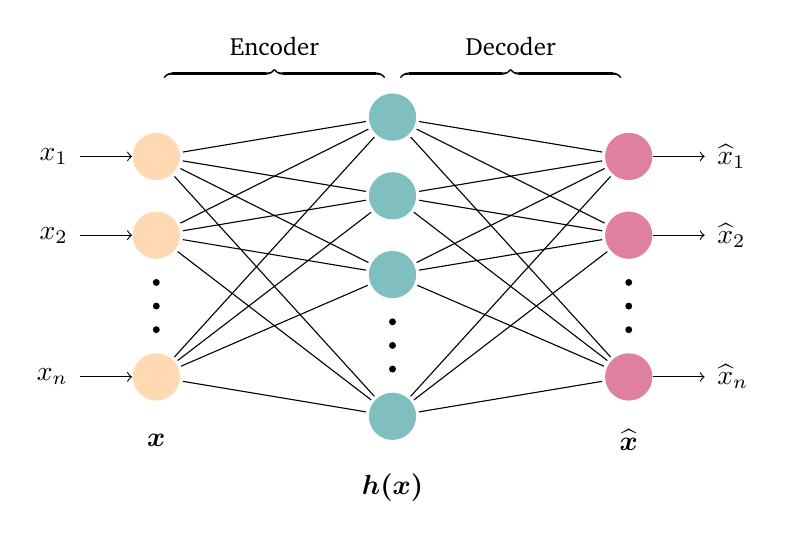
\begin{tikzpicture}
    % Input layer neurons'number
    \newcommand{\inputnum}{2}
    % Hidden layer neurons'number
    \newcommand{\hiddennum}{3}
    % Output layer neurons'number
    \newcommand{\outputnum}{\inputnum}
    % Dotsize
    \newcommand{\dotsize}{1.25pt}
    % xdiff
    \newcommand{\xdiff}{3}
    % Neurons
    \tikzstyle{place}=[circle, draw=black, minimum size = 8mm]
    \tikzstyle{neuron}=[circle, minimum size = 6mm, inner sep = 0]
    % Input Layer
    \foreach \i in {1,...,\inputnum}
      % \foreach \i in {1,2,missing,3}
      {
        \node[neuron][
          fill=orange!30] (Input-\i) at (0,-\i) {};
      }
    % Dots
    \foreach \x in {1,...,3}
      {
        \fill (0, -\inputnum -\x*0.3 - 0.3) circle (\dotsize);
      }
      % Last node
      {
        \node[neuron][
          fill=orange!30] (Input-last) at (0,-\inputnum -0.3*4 - 2*0.3) {};
      }

    % Hidden Layer
    \foreach \i in {1,...,\hiddennum}
      {
        \node[neuron][
          fill=teal!50,
          yshift=(\hiddennum-\inputnum)*5 mm
        ] (Hidden-\i) at (\xdiff,-\i) {};
      }
    % Dots
    \foreach \x in {1,...,3}
      {
        \fill[yshift=(\hiddennum-\inputnum)*5 mm]
        (\xdiff, -\hiddennum -\x*0.3 - 0.3) circle (\dotsize);
      }
      % Last node
      {
        \node[neuron][
          yshift=(\hiddennum-\inputnum)*5 mm,
          fill=teal!50] (Hidden-last) at (\xdiff,-\hiddennum -0.3*4 - 2*0.3) {};
      }

    % Output Layer
    \foreach \i in {1,...,\outputnum}
      {
        \node[neuron][
          fill=purple!50,
          yshift=(\outputnum-\inputnum)*5 mm
        ] (Output-\i) at (2*\xdiff,-\i) {};
      }
    % Dots
    \foreach \x in {1,...,3}
      {
        \fill[yshift=(\outputnum-\inputnum)*5 mm] (2*\xdiff, -\outputnum -\x*0.3 - 0.3) circle (\dotsize);
      }
      % Last node
      {
        \node[neuron][
          yshift=(\outputnum-\inputnum)*5 mm,
          fill=purple!50,] (Output-last) at (2*\xdiff,-\outputnum -0.3*4 - 2*0.3) {};
      }

    % Connect neurons In-Hidden
    \foreach \i in {1,...,\inputnum}
      {
        \foreach \j in {1,...,\hiddennum}
          {
            \draw[-, shorten >=1pt, shorten <=1pt] (Input-\i) -- (Hidden-\j);
          }
      }
    % Input-last to hidden
    \foreach \j in {1,...,\hiddennum}
      {
        \draw[-, shorten >=1pt, shorten <=1pt] (Input-last) -- (Hidden-\j);
      }
    % Hidden-last to input
    \foreach \i in {1,...,\inputnum}
      {
        \draw[-, shorten >=1pt, shorten <=1pt] (Input-\i) -- (Hidden-last);
      }
    % Input-last to Hidden-last
    \draw[-, shorten >=1pt, shorten <=1pt] (Input-last) -- (Hidden-last);

    % Connect neurons Hidden-Out
    \foreach \i in {1,...,\hiddennum}
      {
        \foreach \j in {1,...,\outputnum}
          {
            \draw[-, shorten >=1pt, shorten <=1pt] (Hidden-\i) -- (Output-\j);
          }
      }
    % Hidden to Output-last
    \foreach \i in {1,...,\hiddennum}
      {
        \draw[-, shorten >=1pt, shorten <=1pt] (Hidden-\i) -- (Output-last);
      }
    % Hidden-last to output
    \foreach \j in {1,...,\outputnum}
      {
        \draw[-, shorten >=1pt, shorten <=1pt] (Hidden-last) -- (Output-\j);
      }
    % Hidden-last to Output-last
    \draw[-, shorten >=1pt, shorten <=1pt] (Hidden-last) -- (Output-last);

    % Inputs
    \foreach \i in {1,...,\inputnum}
      {
        \draw[<-, shorten >=1pt] (Input-\i) -- ++(-1,0)
        node[left]{$x_{\i}$};
      }
      {
        \draw[<-, shorten >=1pt] (Input-last) -- ++(-1,0)
        node[left]{$x_{n}$};
      }

    % Outputs
    \foreach \i in {1,...,\outputnum}
      {
        \draw[->, shorten >=1pt] (Output-\i) -- ++(1,0)
        node[right]{$\widehat{x}_{\i}$};
      }
      {
        \draw[->, shorten >=1pt] (Output-last) -- ++(1,0)
        node[right]{$\widehat{x}_{n}$};
      }

    % Bottom text
    \node at (0, -4.6) [black, ] {$\bm{x}$};
    \node at (\xdiff, -5.2) [black, ] {$\bm{h(x)}$};
    \node at (2*\xdiff, -4.6) [black, ] {$\bm{\widehat{x}}$};

    \newcommand{\xmargin}{0.1}
    % curly braces
    \draw[thick,decorate,decoration={calligraphic brace,amplitude=3pt}]
    (0 + \xmargin, 0) coordinate (Input-1) {} --
    (\xdiff - \xmargin, 0) coordinate (Hidden-1) {};
    % curly braces
    \draw[thick,decorate,decoration={calligraphic brace,amplitude=3pt}]
    (\xdiff + \xmargin, 0) coordinate (Hidden-1) {} --
    (2*\xdiff - \xmargin, 0) coordinate (Output-1) {};
    % encoder
    \node at (\xdiff/2, 0.4) [black, ] {\small Encoder};
    % decoder
    \node at (\xdiff + \xdiff/2, 0.4) [black, ] {\small Decoder};
  \end{tikzpicture}
  \caption{Basic autoencoder network architecture with one hidden layer.}
  \label{fig:model}
\end{figure}

The seminal example of an unsupervised model is the \textbf{autoencoder}. It is composed of an \textbf{encoder} part which projects the input to a (often lower-dimensional) hidden representation, and a \textbf{decoder} part which is responsible for turning that representation back into the input vector. A basic autoencoder architecture with a single hidden layer can be seen in figure \ref{fig:model}. By limiting the size of the hidden layer or by imposing restrictions on the gradient through \textit{regularization}, the learned representation can be chosen to have specific desirable properties \cite{Goodfellow-et-al-2016}.

\subsection{Denoising autoencoders}

One such autoencoder model with special properties is called the \textbf{denoising autoencoder} (DAE). Instead of being presented with a sample $\bm{x} \in \mathcal{X}$ as input, it receives a \textit{corrupted version} $\bm{\tilde{x}}$. The loss is still computed with respect to the original, uncorrupted training vector, and so the model effectively learns to remove the noise from the noisy samples, hence the name ``denoising''. Given enough time, it learns the reconstruction distribution $p(\bm{x} \mid \bm{\tilde{x}})$ which is robust to small input perturbations. Mathematically speaking, a traditional autoencoder attempts to minimize the function

\begin{equation}
  \mathcal{L}(\bm{x},\ g(f(\bm{x})))
\end{equation}

\noindent where $\mathcal{L}$ is a specific loss function, and $f$ and $g$ are the functions learned by the encoder and decoder parts of the network respectively. Instead, a DAE minimizes the function

\begin{equation}
  \mathcal{L}(\bm{x},\ g(f(\bm{\tilde{x}})))
\end{equation}

\noindent where $\bm{\tilde{x}}$ is a copy of $\bm{x}$ corrupted by some form of noise. The addition of noise reduces the risk that the model simply learns the \textit{identity function}, which is almost always undesirable. This risk can be further lowered by adding a \textit{penalty term} to the loss function:

\begin{equation}
  \mathcal{L}(\bm{x},\ g(f(\bm{\tilde{x}}))) + \Omega(\bm{\theta})
\end{equation}

\noindent where $\bm{\theta}$ denotes the parameters of the model. This term can take a variety of forms, but in this work it was used to perform $L2$ regularization, also known as \textbf{ridge regression}. The penalty term then takes the following form:

\begin{equation}
  \Omega(\bm{\theta}) = \lambda \sum_i \theta_i^2
\end{equation}

\noindent where $\lambda$ is a coefficient controlling the strength of the regularization. This penalty was added to reduce the chances of overfitting.

The denoising nature of the network makes it robust to small perturbations in the input space. A consequence of this is that any fixed point $x$ of the model will have a surrounding neighborhood of points that can map to $x$, and not just $x$ itself. What this means and how it influences our chosen methodology will now be addressed from the perspective of dynamical systems.

\section{Dynamical systems}

We now introduce a few concepts from the study of dynamical systems that are used in this work to analyze artificial neural networks. For an exhaustive overview of the subject, one can refer to the work `Nonlinear dynamics and Chaos' \cite{strogatz1994nonlinear}.

\subsection{Iterative fixed points}

A \textit{fixed point} of a function $f$ is defined as a point $x$ for which $f(x) = x$. While an autoencoder learns to minimize the reconstruction loss between the input data and their predictions, in reality the training examples are rarely perfectly retrieved after training; instead being close to but almost never exactly equal to the original input.

For this reason, we introduce the concept of \textit{iterative fixed points}. This concept is partially inspired by the recirculation algorithm first proposed in \cite{hinton1987learning}, although importantly the models used in this work are still trained through backpropagation. Because an autoencoder has an input dimension $d$ equal to its output dimension $d_{\rm o}$, model predictions can be reused as input in a sequential fashion. The successive application of a model to an input vector is a process we will refer to as \textbf{iteration}.

\begin{definition}
  Let $f_{\bm{\theta}} : \mathbb{R}^d \rightarrow \mathbb{R}^d$ be the function learned by a $d-$dimensional autoencoder trained on a dataset $\mathcal{X}$. We say that a point $x$ is an \textbf{iterative fixed point} if successive applications of $f_{\bm{\theta}}(\cdot)$ given an initial input of $x$ eventually converge to $x$. This trivially holds for $\forall x \in \mathcal{X}$ given that the model is overparameterized and trained until the loss is sufficiently small.
\end{definition}

\noindent An example of the latter condition not being met can be seen in figure \ref{fig:fixed}, where not all training examples are stored as iterative fixed points in a model where the hidden dimension is constrained.

\begin{figure}%
  \centering
  \subfloat[][\centering Iterating the \textit{Canary} item results in itself]{{
        \includegraphics[width=.25\textwidth]{fixed_point_fromcanary_noadded.pdf}
        \label{fig:fixed:canary}
      }}%
  \qquad
  \subfloat[][\centering \dots while \textit{Pine} instead transitions to \textit{Oak} after iteration]{{
        \includegraphics[width=.25\textwidth]{fixed_point_frompine_noadded.pdf}
        \label{fig:fixed:pine}
      }}%
  \caption{In this particular instance of an underparameterized model, the \textit{Canary} item is stored as an iterative fixed point, while \textit{Pine} is not.}%
  \label{fig:fixed}%
\end{figure}

Using this definition, we can talk about fixed points even though the model doesn't always learn to perfectly memorize the input dataset. The nature of the denoising autoencoder allows us to further expand this concept to the more general notion of \textit{attractors}.

\subsection{Attractors}

Fixed points are merely points that map to themselves, without revealing much about the neighborhood they find themselves in. For example, a saddle point of a function can be an iterative fixed point if approached from the right direction, while any small perturbation in another direction would cause the iteration to diverge. This is an example of an \textit{unstable equilibrium}. The notion of an \textit{attractor} imposes an additional criterium on a fixed point concerning their stability. In this paper, we use following definition of an attractor:

\begin{definition}
  A fixed point $x$ is said to be an \textbf{attractor} if there exists a neighborhood of $x$, $N$, such that for every point $x_N \in N$ the sequence $\{f^k_{\bm{\theta}}(x_N)\}_{k\in \mathbb{N}}$ converges to $x$ as the number of iterations $k \rightarrow \infty$.
\end{definition}

\begin{remark}
  This definition applies to both ``regular'' as well as iterative fixed points.
\end{remark}

\noindent For the sake of identifying attractors, we use the equivalent condition presented in \cite{strogatz1994nonlinear} that a fixed point $x$ can be said to be an attractor if the largest eigenvalue of the Jacobian $\mathbf{J}$ of $f_{\bm{\theta}}$ at point $x$ is strictly less than $1$.

From these definitions, it follows that it is possible to iteratively recirculate the previous output of a model starting from some perturbed training input $\bm{\tilde{x}}$, lying in the so-called \textit{basin of attraction} of $\bm{x}$, to retrieve the original training pattern $\bm{x}$ given that the number of iterations is large enough. By traversing the phase space of the model from an initial vector constrained to the input space of the training set $\mathcal{X}$, the training examples that are stored as attractors can ultimately be retrieved.

\section{Methods}

To study the efficacy of using replay to train a student model, a total of four autoencoder models were built in and trained using Python and the PyTorch framework \cite{paszke2019pytorch}, distributed over two different scenarios. In the first scenario, both models are overparameterized, while in the second scenario, the first model was underparameterized and the second one is overparameterized.

\subsection{Dataset}

The first model was trained to reproduce a hierarchical binary dataset adapted from \cite{rogers2004semantic}, the statistics of which can be seen in figure \ref{fig:data}. The used dataset contained $8$ different items: \textit{Oak}, \textit{Pine}, \textit{Daisy}, \textit{Rose}, \textit{Salmon}, \textit{Sunfish}, \textit{Canary} and \textit{Robin}. Each item had a dimension of $9$, where entries of $0$ or $1$ coded for the attributes \textit{Move}, \textit{Fly}, \textit{Swim}, \textit{Bark}, \textit{Petals}, \textit{Roots}, \textit{Oak}, \textit{Pine}, \textit{Daisy}, \textit{Rose}, \textit{Salmon}, \textit{Sunfish}, \textit{Canary} and \textit{Robin}. The last $8$ dimensions individually code for only a single item, and are essentially just the $8 \times 8$ identity matrix.

\begin{figure}%
  \centering
  \subfloat[][\centering Hierarchical relations]{{
        \includegraphics[width=.245\textwidth]{hierarchy_best.pdf}
        \label{fig:data:hierarchy}
      }}%
  % \qquad
  \subfloat[][\centering Correlation matrix]{{
        \includegraphics[width=.3\textwidth]{correlation_matrix_FINAL.pdf}
        \label{fig:data:correlation_matrix}
      }}%
  \subfloat[][\centering Items and attributes]{{
        \includegraphics[height=.245\textwidth]{dataset_FINAL.pdf}
        \label{fig:data:dataset}
      }}%
  \caption{Category structure in the used hierarchical dataset adapted from \cite{rogers2004semantic}. The dataset has a shape of $(8,\ 9)$, and contains multiple levels of hierarchy as is visible in the correlation matrix.}%
  \label{fig:data}%
\end{figure}

This is an example of how some attributes carry a larger amount of information about the dataset than others, and the expectation is that a model constrained in size will gradually drop these dimensions in favor of those that allow the discrimination of more items. This measure of information content can be more intuitively explained by the \textbf{singular value decomposition} of the dataset $\mathcal{X}$. It is a matrix factorization which decomposes an $m \times m$ matrix into three matrices of size $m \times m$, $m \times n$ and $n \times n$ respectively (examples of which are shown in figure \ref{fig:svd}) and is described by the following equation:

\begin{equation}
  \bm{\mathcal{X}} = \bm{U}\bm{\Sigma}\bm{V^T} = \sum_{i=1}^N \sigma_i\bm{u}^i\bm{v}^{iT}
\end{equation}

\begin{figure}
  \centering
  \includegraphics[width=\linewidth]{svd_new_FINAL.pdf}
  \caption{Singular value decomposition of a subset of the training data. Technically speaking, this is the \textit{thin SVD}, where the matrices $\bm{U}$ and $\bm{V}$ contain only the first $k = min(m,\ n)$ columns (the input-output correlation matrix $\bm{\Sigma}^{yx}$ is $m\times n$). The columns of $\bm{U}$ and rows of $\bm{V}$ each form an orthonormal basis. \textit{Note:} in future references, the singular value matrix here shown as $\bm{S}$ is instead called $\bm{\Sigma}$.}
  \label{fig:svd}
\end{figure}

\noindent Each of the three matrices has a distinct semantic interpretation. In the terminology we borrow from \cite{saxe2019a}, the first matrix $\bm{U}$ is also called the \textit{feature synthesizer} vector. It links the attributes of $\mathcal{X}$ to dimensions called \textit{modes}, which encode semantic distinctions. For example, in figure \ref{fig:svd} mode 3 codes for the difference between \textit{Bark} and \textit{Petals}; allowing \textit{Oak} to be discriminated from \textit{Rose}. The second mode captures more information, essentially splitting the dataset between the \textit{Animals} and the \textit{Plants}.

Similarly, the second matrix $\bm{\Sigma}$ is called the \textit{singular value matrix}, and it is a diagonal matrix with ordered values in decreasing intensity. It can be interpreted as a ranking of the information content contained in the specific modes of $\bm{U}$: the first mode is the only one which codes for \textit{Grow}, an attribute which every item in $\mathcal{X}$ possesses, as such it carries the highest information content and also has the largest singular value.

Finally, the third matrix $\bm{V^T}$ of the SVD can be thought of as the \textit{object analyzer vector}, linking individual items (or objects) $\bm{v}^i$ to their respective modes $\bm{u}^i$ coupled by their singular value $\sigma_i$. For example, since mode 3 distinguishes between \textit{Bark} and \textit{Petals}, attributes which only the \textit{Oak} and \textit{Rose} possess respectively, it is in this matrix that their dissimilarity is captured along the \textit{tree-flower} dimension.

As the network gradually learns to reconstruct the dataset $\mathcal{X}$, broader modes (which describe a larger part of $\mathcal{X}$) are expected to arise first, with finer categories following later, if at all. It is our hypothesis that an underparameterized model will not learn to represent the modes which explain the lowest share of the total variance in $\mathcal{X}$.

\subsection{Experimental setup}

Every training epoch, the first model was presented with a specific amount of \textit{items} that possess certain \textit{attributes}, which are represented by binary vectors. During the training a batch size of $4$ was used for both models, meaning that every epoch gradient descent was performed twice, once on each minibatch. Model statistics (such as the loss) were averaged over $25$ model runs to reduce the effect of random initialization. The parameters were initialized by using Xavier Initialization.

The rectified linear unit (ReLU) was used as the activation function, except for after the last hidden layer in the decoder where a Sigmoid nonlinearity was instead used to constrain the output to the interval $[0,\ 1]$, which is the range the dataset spans. In all models a dropout layer with a probability of $0.15$ was used after the input and hidden layers to reduce the probability of overfitting \cite{dropout}. Initially both models also contained batch normalization layers \cite{batch_norm}, but these were discarded as they did not seem to make a meaningful difference in performance. Optimization was performed using the AdamW optimizer, with a learning rate of $10^{-2}$ in all cases. The loss included an $L2$ penalty term with a $\lambda$ of $0.005$. The loss function used was the mean-squared error (MSE), with the reduction set to $sum$ instead of $mean$:

\begin{equation}
  \mathcal{L}(\bm{y}, \bm{\hat{y}}) = \sum_{i=1}^n (y_i - \hat{y}_i)^2
\end{equation}

\noindent The overparameterized model had a hidden size of $32$ and was trained for a maximum of $3500$ epochs, while the underparameterized one had a hidden size of only $2$ units and instead was trained for a maximum of $1500$. These values were chosen after experimentation with early stopping, where models were trained on the dataset until the average loss of all items reached $10^{-3}$, or when the difference between the average loss in one epoch and the next was less than $10^{-4}$, whichever came first. In the overparameterized case, the former criterion tended to be the cause for early stopping, whereas the underparameterized model never satisfied the former condition and so relied on the latter one for training to stop.

After the first model was trained (whether under- or overparameterized), a second model was trained whose size depended on the specific scenario under consideration. It was trained in the same manner as discussed above, except for the input data now being comprised of patterns generated by iterating random noise. From this ``replay'' dataset, $8$ patterns (equal to the number of items in the original dataset) were uniformly picked from the list of patterns every epoch, and presented in batch sizes of $4$ just like before. The process of pattern generation will now be further discussed.

\subsection{Pattern generation}

Once the first model had been trained to a sufficient level, a new dataset was produced through iterating the model from an initial state of random Gaussian noise. At every step, a certain amount of random noise was optionally added to the generated pattern. The expectation behind this is that perturbing the input will increase the probability of a less stable attractor state being reached, biasing the sampled states away from the strongest attractor. The full algorithm is detailed in algorithm \ref{alg:pattern} below, and the motivation behind it will now be explained.

% Algorithm
\algnewcommand\algorithmicinput{\textbf{Input:}}
\algnewcommand\Input{\item[\algorithmicinput]}

\algnewcommand\algorithmicoutput{\textbf{Output:}}
\algnewcommand\Output{\item[\algorithmicoutput]}

\begin{algorithm}
  \caption{The algorithm used for pattern generation.}
  \label{alg:pattern}
  \begin{algorithmic}
    \Input a model $f_{\bm{\theta}}$, the number of patterns $n$, the number of steps $s$, the noise mean $\mu$, the noise standard deviation $\sigma$
    \Output $p$, a list containing $n$ patterns
    \Require $f_{\bm{\theta}}$ is a trained model

    \State $p \gets [\ ]$
    \For{$i \gets 0,n$}
    \State $\bm{x} \gets \bm{U}(a,\ b)$ \Comment{Initialize with uniform noise; $[a,\ b]$ spans the latent space of $f_{\bm{\theta}}$}
    \For{$j \gets 0,s$}
    \State $\bm{y} \gets f_{\bm{\theta}}(\bm{x})$  \Comment{Model prediction for $\bm{x}$}
    \State $\bm{y} \gets \bm{y} + \bm{\mathcal{N}}(\mu,\ \sigma^2)$ \Comment{Optionally inject Gaussian noise}
    \State $\bm{y} \gets max(0,\ min(1,\ \bm{y}))$  \Comment{Ensure $y_i \in [0,\ 1]\ \forall i$, since the dataset is binary}
    \State $\bm{x} \gets \bm{y}$
    \EndFor
    \State $p \gets p \cup [\bm{x}]$
    \EndFor
    \\
    \Return $p$
  \end{algorithmic}
\end{algorithm}

The used algorithm is in many ways similar to a \textbf{Markov chain Monte Carlo} method. As mentioned above, the goal of the sampling with noise is to traverse the phase space of the model in a more ``equal'' manner, biasing it away from the strongest attractors. But the question remains what values for $\mu$ and $\sigma$ constitute this ``equality''. The used values for the mean and standard deviation of the noise during the pattern generation were determined by the following process.

If a second model is to reliably learn the initial dataset $\mathcal{X}$, two characteristics are desirable in the generated dataset used for training the second model. First, the patterns should have a high similarity to the items in $\mathcal{X}$. Second, the relative frequency of the items should be well-balanced; this to ensure a sufficient degree of interleaving such that catastrophic forgetting does not occur. While the first condition can be satisfied by removing the patterns that are sampled during the ``burn-in time'' of the chain, the latter one poses more of a problem. When every training example $x \in \mathcal{X}$ is an attractor, this is not an issue since patterns would occur relative to the strength of their respective attractor, but when items are not stored as an attractor (e.g. in the underparameterized model), they are instead not retrieved through the process of iteration and end up being rare to non-existent in the generated dataset.

In order to include these non-attractor states which are nonetheless part of the dataset we would like the second model to be able to reproduce, it follows that during iteration we should like transitions to occur between items that are categorically similar. If sampling without noise would in large amounts produce the final state of \textit{Oak}, noise-assisted perturbations during iteration should in some cases cause the state to instead jump to the basin of attraction of an item that lies nearby in the latent space, e.g. the \textit{Pine}, even if \textit{Pine} is itself a weak attractor or not an attractor at all. In the latter case, the state representing the item would not be favored over neighboring states that are not in $\mathcal{X}$ at all, and so our expectation is that sampling with noise comes paired with a general degradation in the quality of the produced patterns.

The notion of transitions during the process of iteration is encapsulated by the \textbf{transition matrix}, which captures what outputs certain inputs map (or ``transition'') to after model prediction. If every item is an iterative fixed point and iteration is performed without injecting intermediary noise, this matrix would be equal to the identity matrix with every item always transitioning to itself. The desire that the transition matrix should reflect the category structure of the dataset leads us to posit that the optimal values of $\mu$ and $\sigma$ for the added noise during iteration are those that minimize the difference between the transition matrix and the rescaled correlation matrix seen in figure \ref{fig:data:correlation_matrix}. A transition matrix produced by generating patterns with these ``optimal'' values for $\mu$ and $\sigma$ can be seen in figure \ref{fig:transition_matrix}.

Mathematically, this means the following: let $\mathbf{A}(\mu,\ \sigma)$ be the transition matrix generated by iterating for $n$ runs where $n$ is a large number (e.g. $10000$), and let $\mathbf{S}$ be the Pearson correlation matrix of $\mathcal{X}$ rescaled such that all of its entries lie in the closed interval $[0,\ 1]$. Then the sum of the Hadamard product of the difference between these matrices $\sum (\mathbf{A}(\mu,\ \sigma) - \mathbf{S}) \circ (\mathbf{A}(\mu,\ \sigma) - \mathbf{S})$ has a minimum value, as shown in figure \ref{fig:noise_surf}. These values were found to be very close to $\mu = 0$ and $\sigma = 0.5$, which were the values ultimately chosen for the noisy generation of patterns.

\begin{figure}
  \centering
  \subfloat[][\centering Error surface produced by measuring the dissimilarity between the rescaled correlation matrix of the dataset and the transition matrix at different values of $\mu$ and $\sigma$]{{
        \includegraphics[width=.31\textwidth]{1_over_32_noise_surf_viridis.pdf}
        \label{fig:noise_surf}
      }}%
  % \qquad
  \subfloat[][\centering The rescaled correlation matrix $\mathbf{S}$ used in the calculation of categorical similarity]{{
        \includegraphics[width=.31\textwidth]{dists_normed.pdf}
        \label{fig:resc_corr}
      }}%
  % \qquad
  \subfloat[][\centering An example transition matrix $\mathbf{A}$ after iterating with the ``optimal'' values of $\mu = 0$ and $\sigma = 0.5$]{{
        \includegraphics[width=.31\textwidth]{transition_matrix_FINAL.pdf}
        \label{fig:transition_matrix}
      }}%
  \caption{The existence of a global minimum for $\mu$ and $\sigma$ in the categorical dissimilarity between $\mathbf{A}$ and $\mathbf{S}$, and the corresponding transition matrix. $\bm{A}$ was produced by iterating the trained model according to algorithm \ref{alg:pattern} for $10,000$ runs, and $\bm{S}$ was made by using min-max scaling to rescale the correlation matrix to the interval $[0,\ 1]$.}
\end{figure}

\subsection{Reliability and limitations}
\label{subsec:limitations}

In order to improve reproducibility, the

While we have made the assumption here that pattern generation is optimal for model performance when the transition matrix produced by iteration most accurately reflects the rescaled correlation matrix, it remains to be seen whether this is actually true. Though we did not attempt to provide a quantitative measure for model learning as a function of noise $\mu$ and $\sigma$, it would nevertheless have been interesting to investigate the effects of different noise parameters on the generated set of patterns.

Even though the generated patterns were produced by running $n$ independent chains where $n \sim 10000$, this number might not actually have been large enough to sample the whole state space. Although the results were averaged over $25$ different model runs to increase reliability, the ergodicity of the Markov chain could have been explored to ensure that no path-dependence was influencing the learning of the second model.

\section{Results}

As mentioned before, two scenarios were considered. In the first one, the first model was \textit{underparameterized} with a hidden size of $2$, and in the second one it was \textit{overparameterized} having a hidden size of $32$. In both cases, the second model was overparameterized, also sporting a hidden layer with a code size of $32$.

\subsection{Underparameterized scenario}

The training statistics for the first model being underparameterized can be seen in figure \ref{fig:under}. When the first model is constrained in size, the network is unable to accommodate every dimension in order to fully replicate the dataset, and so it is forced to generalize. This is especially apparent in figure \ref{fig:under:singular}, where the diagonal entries of the singular value matrix $\bm{\Sigma}$ are plotted (produced by decomposing the matrix of model predictions every epoch): only 5 of the total of 8 singular values are nonzero when the model finishes training. The average loss per item hovers around $0.5$ in epoch $1500$, with a large deviation across different model runs. The injection of noise during the sampling process caused the \textit{Rose} and \textit{Pine} items to be included in the replay dataset to a much higher degree, which improved their loss at the expense of the other items.

\begin{figure}%
  \centering
  \subfloat[][\centering Loss curves]{{
        \includegraphics[width=.31\textwidth]{1_under_2.pdf}
        \label{fig:under:loss}
      }}%
  % \quad
  \subfloat[][\centering Individual item losses]{{
        \includegraphics[width=.31\textwidth]{1_under_2_loss_per_item.pdf}
        \label{fig:under:loss_per_item}
      }}%
  % \quad
  \subfloat[][\centering Singular value trajectories]{{
        \includegraphics[width=.31\textwidth]{1_under_2_singular_magma.pdf}
        \label{fig:under:singular}
      }}%
  \caption{Training metrics for an \textit{underparameterized} first model with a hidden size of 2, averaged over 25 model runs. Because of limited capacity, the network is forced to generalize, which is visible in the large deviations in individual item losses between model runs, and also in the small amount of nonzero singular values.}%
  \label{fig:under}%
\end{figure}

Since the underparameterized has a code size of only $2$ dimensions, we can directly visualize its latent space without having to resort to dimensionality reduction. This visualization highlighting the existence of attractors can be seen in figure \ref{fig:singlet_attr}.

\begin{figure}
  \centering
  \includegraphics[width=.8\linewidth]{in_depth_attr.pdf}
  \caption{Visualization of the latent space learned by an underparameterized first model. Not every item is stored as an attractor, and some representations heavily overlap. This plot was produced by generating a grid of $10,000$ $2d$ points and feeding it only through the decoder part of the network, after which they were categorized as the item that was closest (measured by Euclidean distance) to the model prediction and colored appropriately. The arrows stem from iterating each point for $25$ steps and computing the difference between start and end states in the hidden layer; their magnitudes are proportional to the distance covered. The stars represent the hidden encodings of the items $\bm{x} \in \mathcal{X}$.}
  \label{fig:singlet_attr}
\end{figure}

Training metrics for the second (overparameterized) model when trained on patterns sampled from the first, underparameterized one can be seen in figure \ref{fig:under_over_sample}. These metrics were also averaged over $25$ model runs, although the observed variation is much smaller.

\begin{figure}%
  \centering
  \subfloat[][\centering Loss curves for the second model when training patterns are sampled without noise]{{
        \includegraphics[width=.31\textwidth]{2_over_1_under_2_nonoise.pdf}
        \label{fig:under_over_sample:nonoise}
      }}%
  % \quad
  \subfloat[][\centering Loss curves for the second model when trained on patterns generated with a noise level of $\mu=0$ and $\sigma=0.5$]{{
        \includegraphics[width=.31\textwidth]{2_over_1_under_2_noise_std_0,5.pdf}
        \label{fig:under_over_sample:noise}
      }}%
  % \quad
  \subfloat[][\centering Relative increase of sampled patterns when noise is used]{{
        \includegraphics[width=.31\textwidth]{2relative_increase_avg_over_25_1_under_2_over.pdf}
        \label{fig:under_over_sample:rel_inc}
      }}%
  \caption{The addition of noise during the sampling process increases the prevalence of certain items in the replay dataset, causing them to be learned better at the expense of other items.}%
  \label{fig:under_over_sample}%
\end{figure}

\subsection{Overparameterized scenario}

In this scenario, both models were overparameterized. The relevant training curves are visible in figure \ref{fig:over}. While the model was trained for a total of $1500$ epochs, the plots are constrained to $t \in [0,\ 150]$ to increase visibility; all loss curves eventually approach $0$ as $t$ goes beyond $150$. Only $6$ out of $8$ singular values are nonzero after training.

\begin{figure}%
  \centering
  \subfloat[][\centering Loss curves]{{
        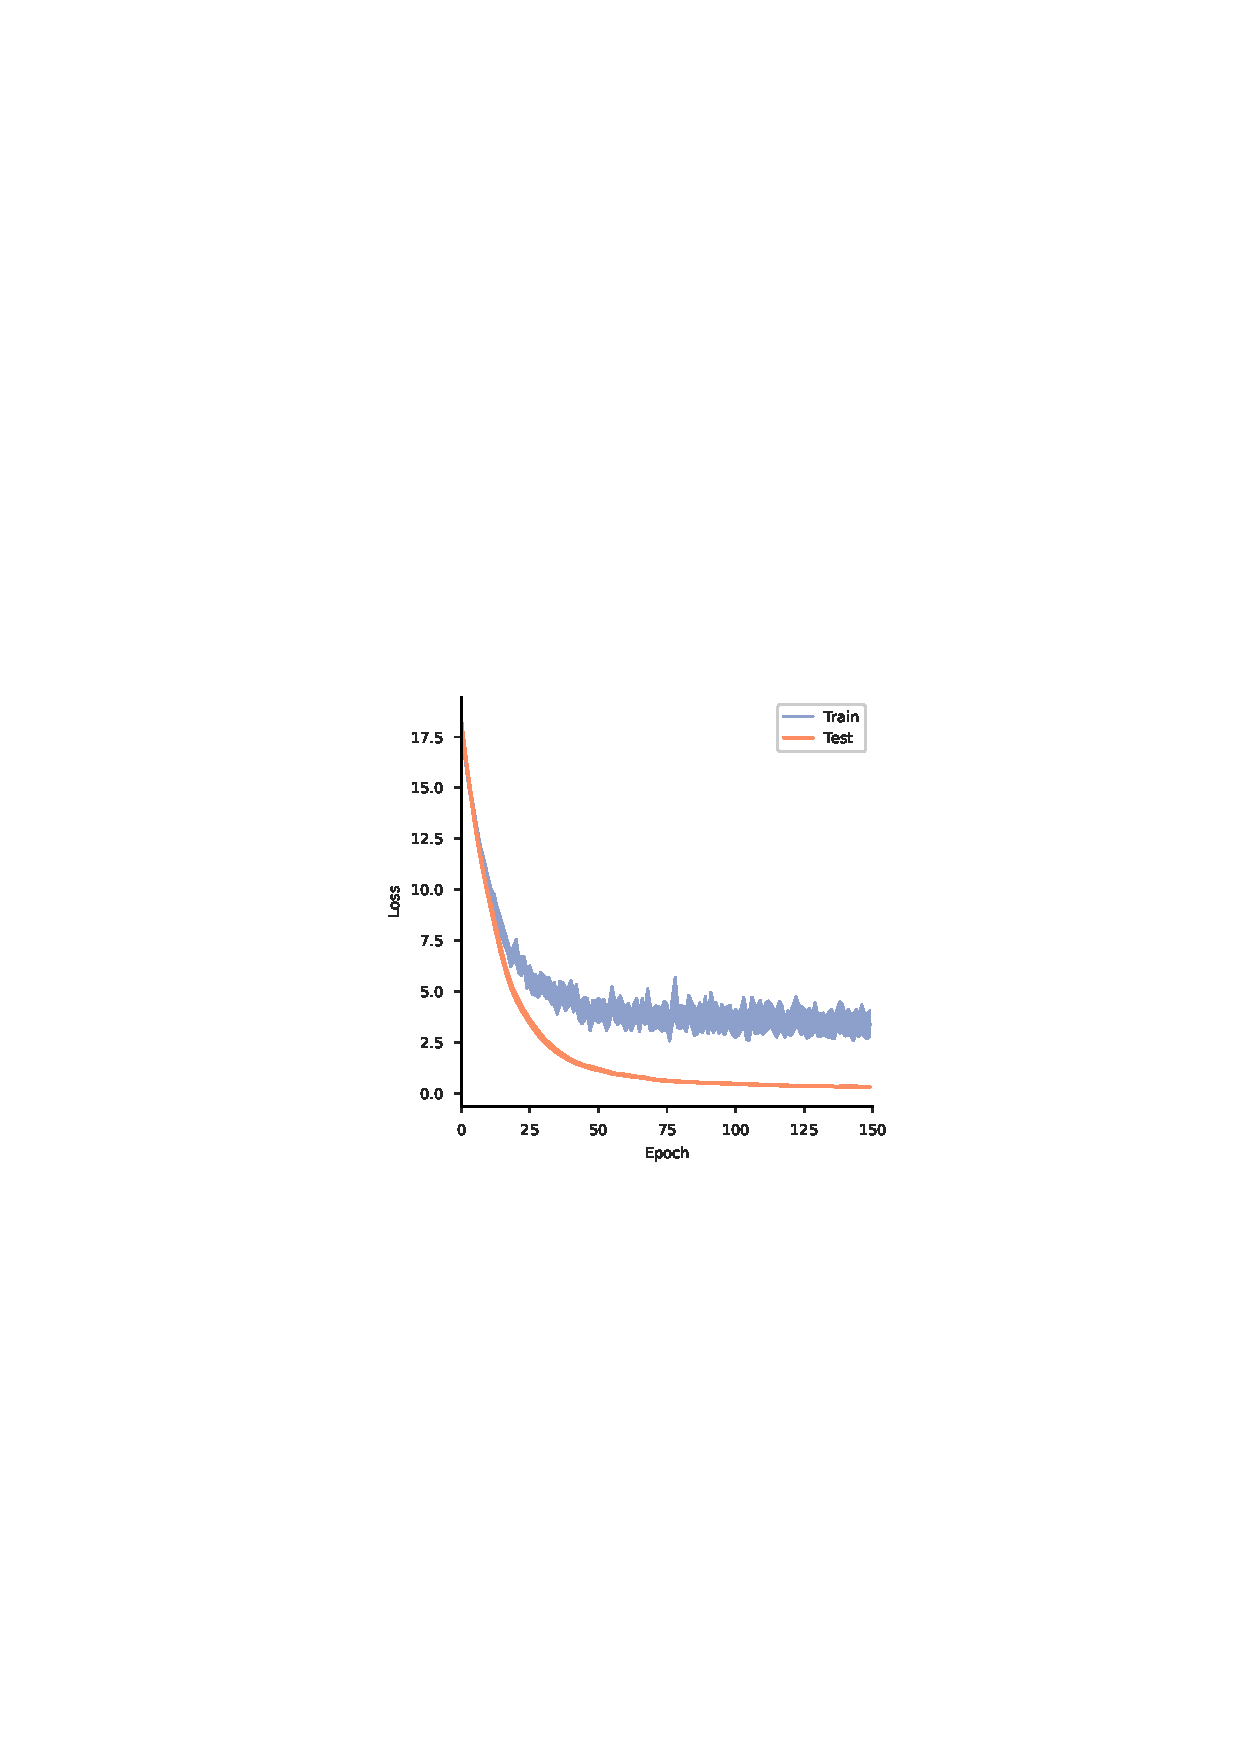
\includegraphics[width=.31\textwidth]{1_over_32.pdf}
        \label{fig:over:loss}
      }}%
  % \quad
  \subfloat[][\centering Individual item losses]{{
        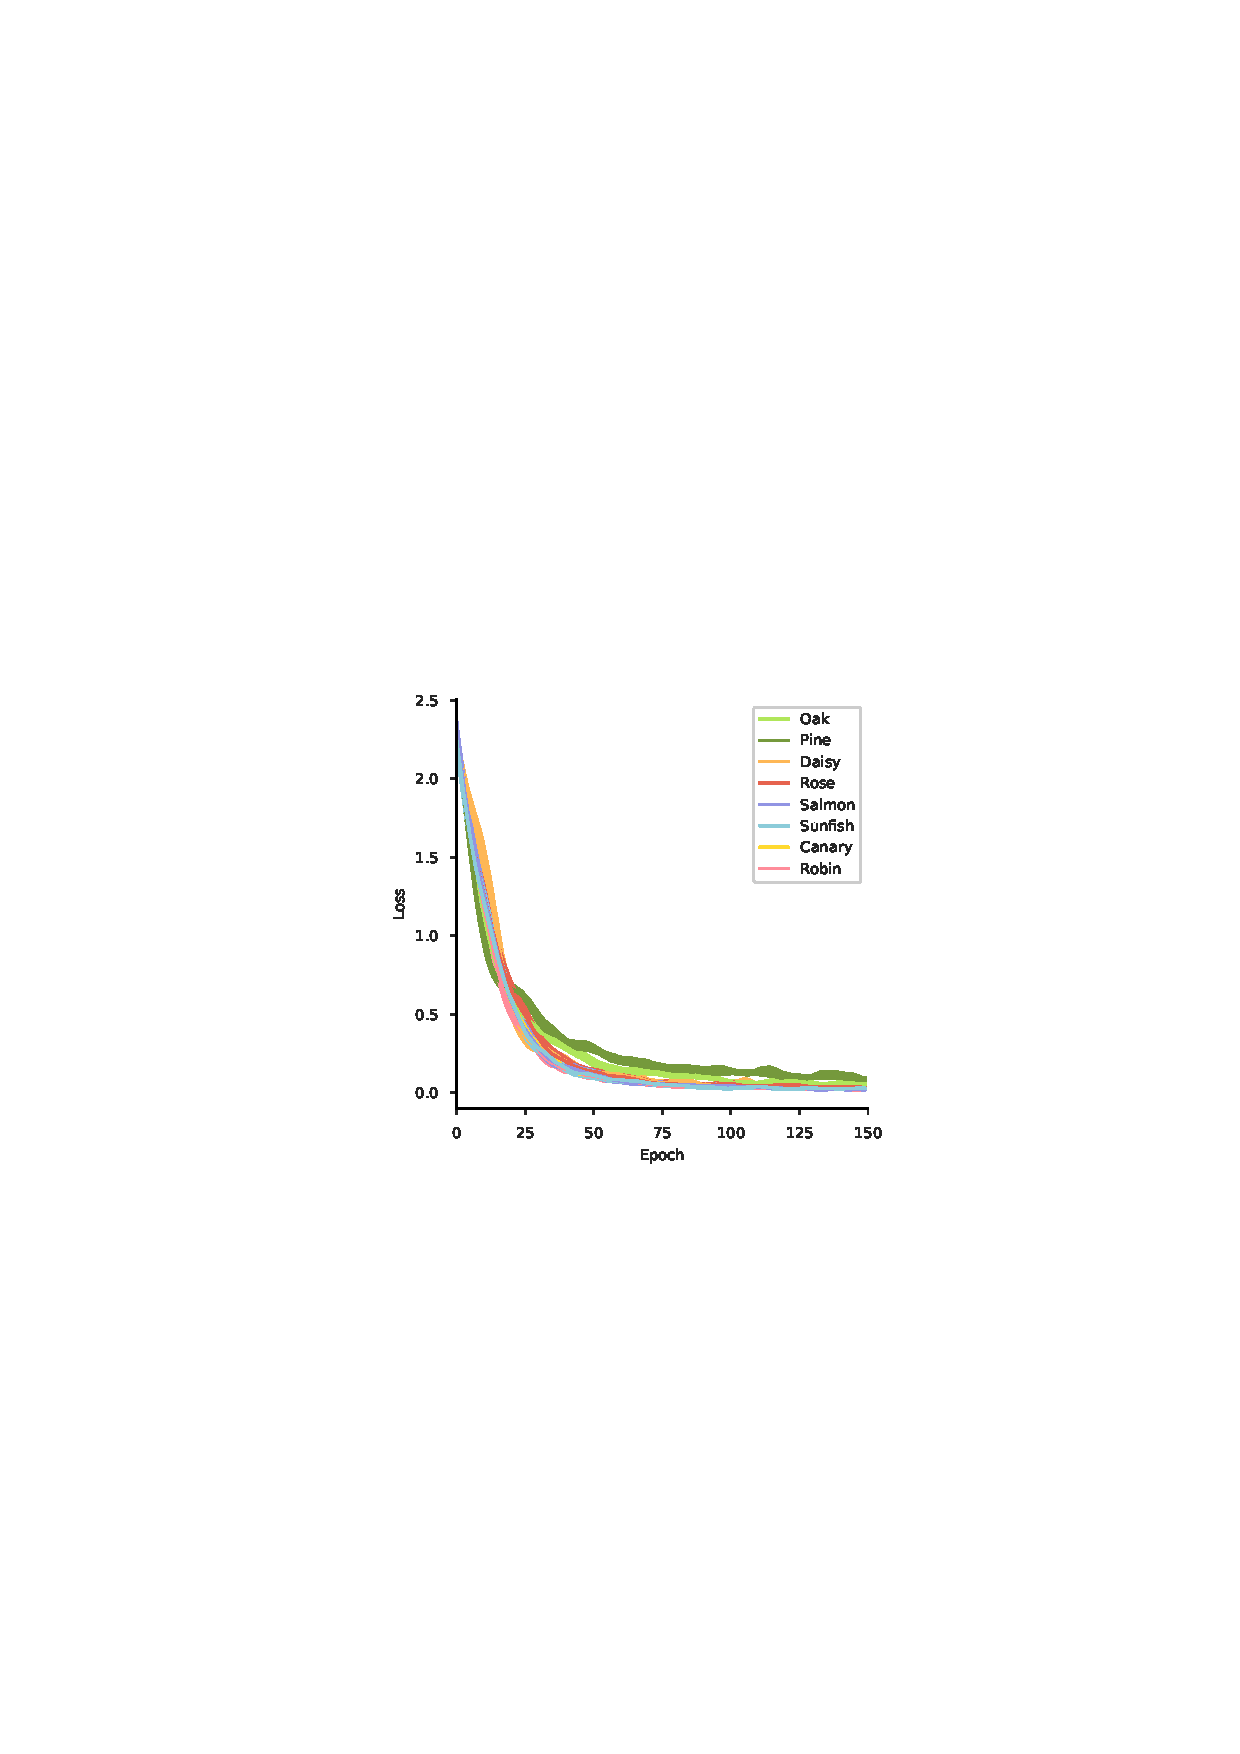
\includegraphics[width=.31\textwidth]{1_over_32_loss_per_item.pdf}
        \label{fig:over:loss_per_item}
      }}%
  % \quad
  \subfloat[][\centering Singular value trajectories]{{
        \includegraphics[width=.31\textwidth]{1_over_32_singular_magma.pdf}
        \label{fig:over:singular}
      }}%
  \caption{Training metrics for an \textit{overparameterized} first model with a hidden size of 32. In a short amount of time, all items are able to approach a loss of 0.}%
  \label{fig:over}%
\end{figure}

In parallel to figure \ref{fig:singlet_attr} produced for the underparameterized model, figure \ref{fig:triplet_attr} attempts to do the same for the overparameterized one, with the important distinction that PCA is now performed on the hidden dimension of size $32$ instead of it directly corresponding to the latent space. The explained variance of the three plotted PCA dimensions was $0.58$, $0.21$ and $0.12$ for each dimension respectively (in ascending order), for a total of $0.91$.

\begin{figure}
  \centering
  \includegraphics[width=\linewidth]{1_over_32_attr_grid_triplet_legend_2.pdf}
  \caption{The existence of iterative fixed points and their basins of attraction in the latent space of an overparameterized model with a hidden size of 32. The explained variance by the PCA dimensions were $0.58$, $0.21$ and $0.12$ respectively, adding up to $0.91$. Note that some stars (representing the items) lie in areas of a different color; this is due to the grid points being passed through the \textit{decoder} and colored based on the prediction, whereas the items were only passed through the \textit{encoder} to get their position in the latent space. Passing the point corresponding to the item through the decoder too would classify it according to the background color of the points around it.}
  \label{fig:triplet_attr}
\end{figure}

Similarly, the three plots in figure \ref{fig:over_over_sample} convey the same information as figure \ref{fig:under_over_sample} did for the previous scenario. The addition of noise degrades the quality of the patterns to a lesser extent compared to the sampling performed on the underparameterized model.

\begin{figure}%
  \centering
  \subfloat[][\centering Loss curves for the second model when training patterns are sampled without noise]{{
        \includegraphics[width=.31\textwidth]{2_over_1_over_32_nonoise.pdf}
        \label{fig:over_over_sample:nonoise}
      }}%
  % \quad
  \subfloat[][\centering Loss curves for the second model when trained on patterns generated with a noise level of $\mu=0$ and $\sigma=0.5$]{{
        \includegraphics[width=.31\textwidth]{2_over_1_over_32_noise_std_0,5.pdf}
        \label{fig:over_over_sample:noise}
      }}%
  % \quad
  \subfloat[][\centering Relative increase of sampled patterns when noise is used]{{
        \includegraphics[width=.31\textwidth]{relative_increase_avg_over_5.pdf}
        \label{fig:over_over_sample:rel_inc}
      }}%
  \caption{Even when the first model is overcomplete, a second model can occasionally fail to learn specific items when trained on sampled patterns. The addition of noise can improve the general performance of the second model.}%
  \label{fig:over_over_sample}%
\end{figure}

\section{Discussion}

\textbf{Injecting noise during the sampling process improved the prevalence and learning of underrepresented items.} In general, it seems that the injection of noise during the pattern generation process allows some items to be learned to a much higher degree, at the cost of degrading the general quality of the predictions. Remarkably, this phenomenon occurred for \textit{both} the under- and overparameterized networks, although the pattern quality was much worse in the underparameterized scenario. This is surprising since the underparameterized model is only able to store very few attractors, as visible in figure \ref{fig:singlet_attr}, and so sampling was not predicted to produce the same effect as for the overparameterized model. Our hypothesis is that the closeness of the items in the latent space and their position within the basin of attraction of an attractor, even if they are not one themselves, accounts for their increased prevalence in the replay dataset. This may be due to the step size of the Markov chain being too small for the state to converge to the global minimum.
\\
\\
\textbf{Overlap in the 2d latent space.} As can be seen in figure \ref{fig:singlet_attr}, the underparameterized model only (in general) had 3 attractor states in its latent space, none of which corresponded exactly to an item from the dataset. For example, \textit{Oak}, \textit{Pine} and \textit{Daisy} are tightly grouped in the leftmost attractor, while \textit{Rose} occupies an area further away in the basin. \textit{Salmon} and \textit{Robin} share an attractor, as do \textit{Canary} and \textit{Sunfish}, suggesting that the \textit{red-yellow} mode capturing the color has come to dominate the learning over the \textit{animal-plant} dimension.
\\
\\
\textbf{Memorization in the overparameterized latent space.} While the multidimensional nature of the hidden space makes it difficult to see in figure \ref{fig:triplet_attr}, all items \textit{except} for \textit{Pine} are memorized as attractors in the overparameterized first model. Remarkably, \textit{Pine} and \textit{Oak} were never stored as individual attractors in any of our experiments and instead always shared a common one. This is probably due to them being the most related items in the dataset, as can be glanced from the correlation matrix in figure \ref{fig:data:correlation_matrix}.
\\
\\
\textbf{Low individual loss does not entail attractor status.} From figure \ref{fig:under:loss_per_item}, it appears that the \textit{Rose} item is able to consistently achieve a much lower than average loss. It is therefore quite surprising to see that it actually lies the \textit{furthest} away from an attractor state in the latent space in figure \ref{fig:singlet_attr} compared the rest. From this, we can conclude that an item having low loss does not justify the prediction that it also encodes an attractor state in the latent space, something which seems like a reasonable expectation.
\\
\\
\textbf{Every fixed point is also an attractor.} All of the iterative fixed points were found to be attractors after evaluation of their Jacobians. In an exploratory analysis, fixed points which were \textit{not} attractors only arose for a large hidden dimension ($\geq$ 64). Interestingly, \textit{spurious attractors} (attractor states $\notin \mathcal{X}$ in an overparameterized model) also started to appear at this level of network capacity.
\\
\\
\textbf{Differences between the singular values.} While the underparameterized model is seen to only have $5$ nonzero singular values after training (figure \ref{fig:under:singular}), the overparameterized model has $6$ nonzero entries, an increase of only $1$ which still leaves $2$ dimensions as being irrelevant for model prediction. Upon closer inspection, these two ignored modes were found to code for the \textit{Grow} attribute and the set of attributes which coded only for individual items. While the mode which encodes \textit{Grow} is associated with the \textit{largest} singular value in figure \ref{fig:svd}, it explains $0$ variance when discriminating between items, since every item possesses this attribute. This matches our expectations for the learning dynamics.

\section{Conclusions}

In this paper, we have shown that a second student model is able to learn an initial hierarchical dataset by training on replayed patterns generated by iterating a first teacher model, which is trained on the dataset, starting from random, uniform noise. Through the intermediate injection of Gaussian noise, this process can be biased away from strong attractors, producing a dataset more fitting for the equal learning of items. We have detailed a general process for navigating the state space of a model in order to sample attractor states, and posited that there exists an optimal noise level for the injections, achieved when the transition matrix produced by iteration most resembles the category structure of the data, which benefits the learning of the second model the most.

While the implications of this may not be significant in terms of model performance given that the second model did suffer a reasonable penalty in accuracy when noise was injected, a way to retrieve knowledge stored in the weights of a model in an unsupervised manner might be interesting for the further study of generative replay from a connectionist standpoint.

\section{Recommendations}

We now make some recommendations for further work concerning this subject.
\\
\\
\noindent \textbf{Different model architectures.} Experimentation with different model architectures is an obvious avenue to pursue. Model depth and layer width can be varied (this work only considered shallow autoencoders with 1 hidden layer), or completely different architectures could be explored. While DAEs incentivize the reconstruction function to resist small but finite-sized perturbations of the input, \textbf{contractive autoencoders} instead bestow this property on to the function responsible for feature extraction. This makes the latent space \textit{locally contractive}, a characteristic which might influence attractor formation. Another interesting direction is that of \textbf{variational autoencoders}, which learn a multivariate normal distribution that best captures the training set. They are inherently generative, and their probabilistic nature makes them much easier to sample patterns from.
\\
\\
\noindent \textbf{Optimal noise level.} As mentioned in subsection \ref{subsec:limitations}, it remains to be seen what the actual influence of the noise mean $\mu$ and standard deviation $\sigma$ on the learning actually means quantitatively. Evaluating the patterns and learning produced by varying these values might reveal a more concrete relation between the two.
\\
\\
\noindent \textbf{Quantitative metric for hierarchical learning.} Since the amount of models we used was so small, we used no quantitative metric to capture the quality of learning, however this would be useful for large-scale experimentation and comparison. This could be accomplished by generating large hierarchical datasets through a process like branching diffusion \cite{saxe2019a}, and training many different models in the fashion presented here. The existence of a suitable metric could allow those results to be interpreted in a meaningful way.
\\
\\
\noindent \textbf{Attractor strength and prevalence in sampled patterns.} Lastly, an investigation could be warranted about the potential relationship between attractor strength and the effect the noise injection during the sampling has on the pattern prevalence in the replay dataset. By coupling this with more tests, our hypothesis that noise allows lower-strength attractors to be reached could be confirmed or rejected, since the amount of models used here does not allow such a general relationship to be extrapolated.

% \section*{Acknowledgements}
% i would like to thank my dog

\clearpage

% Bibliography
\bibliographystyle{plain}
\bibliography{bibliography}

% \appendix
% \section{Appendix}

% \subsection{ReLU}

% \subsection{AdamW}

\end{document}
